\chapter{Fault Tolerant Clustering}

The influence of system failures on task clustering has received little attention. However, system failures play an important role in terms of both system reliability and runtime performance of workflow applications. In this chapter, we analyze the influence of different categories of transient failures and then we propose fault tolerant clustering methods to reduce their influence on the overall workflow performance. Simulation-based experiments show that our dynamic reclustering methods can achieve a speedup of up to 5 in the overall runtime of workflows compared to the horizontal clustering without taking fault tolerance into consideration. 

\section{Motivation}

Task clustering is an effective method to reduce scheduling overhead and increase the computational granularity of tasks executing on distributed resources. However, a job composed of multiple tasks may have a greater risk of suffering from failures than a job composed of a single task. In this chapter we indicate that such failures can have a significant impact on the runtime performance of workflows under existing clustering strategies that ignore failures. 

We focus on transient failures because they are expected to be more prevalent than permanent failures \cite{Zhang2004}. Transient failures are random failures and are recoverable. For example, denser integration of semiconductor circuits and lower operating voltage levels may increase the likelihood of bit-flips when circuits are bombarded by cosmic rays and other particles \cite{Zhang2004}. Based on their occurrence, we divide the transient failures into two categories: task failure and job failure. If the transient failure occurs to the computation of a task (task failure), other tasks within the job do not necessarily fail. If the transient failure occurs to the clustered job (job failure), all of its tasks fail. Accordingly, we have two models. In the task failure model (TFM), the failure of a task is a random event that is independent of the workflow characteristics and execution environment (such as which compute node the task is executed on). The task failure rate is the percentage of failed tasks among all executed tasks. Similarly we can define the job failure rate as the percentage of failed jobs among all executed jobs and a job failure model (JFM) in which job failure is a random event. Figure~\ref{fig:ftc_failure} shows a simple example of job failure and task failure, in which we have a clustered job ($j$) with four tasks ($t_1$, $t_2$, $t_3$ and $t_4$). If all of the four tasks fail (the left figure), it is more likely to have a job failure. If only a portion of tasks within a clustered job fail (for example, in the right figure, only $t_1$ and $t_3$ fail), it is more likely to be a task failure. 
%The left job is more likely to have a job failure since all of its tasks fail. The right job is more likely to have two task failures since the other two tasks do not fail. 

With such a classification of failures, we then analyzed their distinct influence on the overall runtime performance. Respectively, we present a job failure model and a task failure model. What distinguishes our work is that: 1) we analyzed the optimal size of a clustered job based on the estimation of failure rate; 2) we dynamically retried clustered jobs based on the suggested optimal size of a clustered job; 3) furthermore, we select more reliable resources to run clustered jobs. 

%We further improve our methods to be able to handle the situations where task failure rate is not fully independent of workflow characteristics or execution environment. Samak \cite{Samak2011} et.al. have analyzed 1,329 real workflow executions across six distinct applications and concluded that the type and the host id of a job are among the most significant factors that impacted failures. Task specific failure is a type of failure that only occurs to some specific types of tasks. Location specific failure only occurs to some specific execution nodes. What is more, we present two refinements to handle the situation when there are fewer jobs than available resources. 

%In this work, we assume that failures can be observed from the outputs or logs of a job. We only focus on transient failures and we assume that after a finite number of retries these jobs can be completed successfully. 
\begin{figure}[h!]
	\centering
    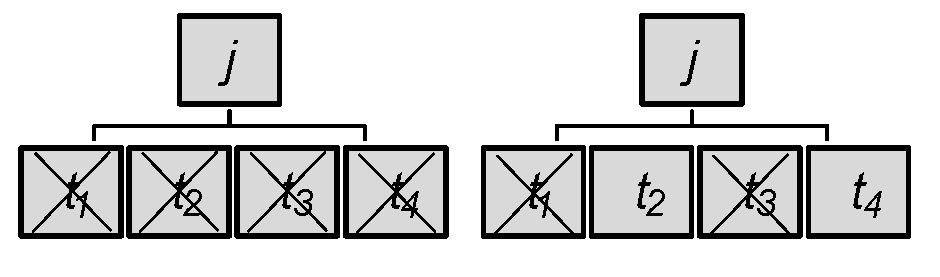
\includegraphics[width=0.6\textwidth]{figures/tolerance/ftc_failure.pdf}
    \caption{Job Failure (Left) and Task Failure(Right). The symbol $\times$ indicates a failure.  }
    \label{fig:ftc_failure}
\end{figure}


\section{Related Work}

%Tang \cite{Tang1990} presented system characteristics such as error and failure distribution and hazard rates. 
Schroeder et al. \cite{Schroeder2006} has studied the statistics of the data, including the root cause of failures, the mean time between failures, and the mean time to repair. Sahoo et al. \cite{Sahoo2004} analyzed the empirical and statistical properties of system errors and failures from a network of heterogeneous servers running a diverse workload. Oppenheimer et al. \cite{Oppenheimer2002} analyzed the causes of failures from three large-scale Internet services and the effectiveness of various techniques for preventing and mitigating service failure. 
%McConnel \cite{McConnel} analyzed the transient errors in computer systems and showed that transient errors follow a Weibull distribution. 
Benoit \cite{Benoit2010} et al. analyzed the impact of transient and fail-stop failures on the complexity of task graph scheduling. Our approach is based on these works. We measure the failure rates in a workflow and then provide fault-aware methods to improve task clustering.  

Task retry is a technique that simply retries the failed job until it is successful. However, some of the tasks within the job may have completed successfully and it could be a waste of time and resources to retry all of the tasks. The Recovery-Aware Components approach \cite{Yusuf2009} proposed a purely component-based fault tolerant approach to increase the reliability of grid applications, essentially by predicting possible failures with a proactive Markov model and proactively initiating failure aversion. In our work, we also use task retry to resubmit failed tasks to execute. However, the difference is that we also adjust the size of a clustered job (number of tasks within a job) dynamically in order to optimize the runtime performance. 

Egwutuoha \cite{Egwutuoha2012} proposed to use process level redundancy techniques to reduce the runtime of the execution of computational intensive applications and reduced the overhead associated with checkpointing significantly. The application process can be periodically checkpointed so that when a failure occurs, the amount of work to be retried is limited. However, checkpointing increases the runtime of the execution of applications \cite{Zhang2004}. For a large workflow with many short tasks, the overheads of checkpointing can still limit its benefits. The difference is that we only check the completion status of a job after a job is completed and resubmit it if it failed. This approach avoids frequent checkpointing since most tasks are short and thus we can reduce the overheads of task retry. 

Kwok \cite{Kwok2000} proposed to use a duplication-based approach in scheduling tasks to a heterogeneous cluster of PCs. In duplication-based scheduling, critical tasks are redundantly scheduled to more than one machine in order to reduce the number of inter-task communication operations. The task duplication process is guided by the system heterogeneity in that the critical tasks are scheduled or replicated in faster machines. Meyer et al. \cite{Meyer2006} presented a generalized approach to planning spatial workflow schedules for Grid execution based on the spatial proximity of files and the spatial range of jobs. They proposed to take advantage of data locality through the use of dynamic replication and schedule jobs in a manner that reduces the number of replicas created and the number of file transfers performed when executing a workflow. 
However, inappropriate clustering (and replication) parameters may cause severe performance degradation if they create long-running clustered jobs. As we will show, a long-running job that consists of many tasks has a higher job failure rate even when the task failure rate is low.   

Silva et al. \cite{Silva2012} presented a self-healing process that quantifies incident degrees of workflow activities from metrics measuring long-tail effect, application efficiency, data transfer issues, and site-specific problems. No strong assumption is made on the task duration or resource characteristics and incident degrees are measured with metrics that can be computed during the runtime. Silva and Rebello \cite{daSilva2011} described a strategy to endow autonomic MPI applications with the property of self-healing and thus be capable of withstanding multiple simultaneous crash faults of processes and/or processors. In our work, we do not categorize the physical causes of a failure since different causes may share the similar influence on the runtime performance of task clustering.  We thus characterize failures in terms of task or job failures since they have totally different influence on the overall runtime. 

\section{Approach}

\subsection{Failure Models}

The goal is to reduce the estimated finish time ($M$) of $n$ tasks in case the failure rate for a clustered job (denoted by $\beta$) or a task (denoted by $\alpha$) is known. $M$ includes the runtime of the clustered job and its subsequent retry jobs if the first try fails. The average time to run a single task once is $\bar{\phi_t}$. $k$ is the cluster size indicating the number of tasks in a clustered job. For a clustered job, let the expectation of retry times to be $N$. The process to run (and retry) a job is a Bernoulli trial with only two results: success or failure. Once a job fails, it will be retried until it is eventually completed successfully because we assume all the failures are transient. By definition we have, $N=1/\gamma=1/(1-\beta)$, while $\gamma$ is the success rate of a job.
Below we show how to estimate $M$. $r$ is the number of available resources. $D$ is the time delay between jobs and it includes the workflow engine delay, the queue delay and the postscript delay. We assume that $n\gg r$, but $n/k$ is not necessarily much larger than $r$. Normally at the beginning of workflow execution, $n/k > r$, which means there are more clustered jobs than available resources. To try all $n$ tasks once irrespective of whether they succeed or fail, one needs approximately $n/(rk)$ execution cycle(s) since at each execution cycle we can execute at most $r$ jobs. Therefore, the time to execute all $n$ tasks once is $n(k\bar{\phi_t}+D+Ck)/(rk)$. And the time to complete them successfully in a faulty environment is $Nn(k\bar{\phi_t}+D+Ck)/(rk)=n(k\bar{\phi_t}+D+Ck)/(rk\gamma)$ since each job requires $N$ retries on average.  
On the other side, at the end of the workflow execution, since $n$ is decreasing with the process of workflow, it is possible that $n/k < r$, which means there are fewer jobs than the available resources. One needs just one execution cycle to execute these tasks once. The time to complete all $n$ tasks successfully is $N(k\bar{\phi_t}+D+Ck)=(k\bar{\phi_t}+D+Ck)/\gamma$. 
Below we discuss how we estimate $\gamma$ in TFM and JFM. In JFM, we have assumed that job failure is an independent event and thereby we only need to collect the failure records of jobs. $\gamma=(1-\beta)$. In conclusion, in JFM, 
\begin{equation} 
\label{eq:jfm}
M=
\begin{cases}
\cfrac{Nn(k\bar{\phi_t}+D+Ck)}{rk}=\cfrac{n(k\bar{\phi_t}+D+Ck)}{rk\gamma}, & \text{if } \cfrac{n}{k}\geq r \\
N(k\bar{\phi_t}+D+Ck)=\cfrac{k\bar{\phi_t}+D+Ck}{\gamma}, & \text{else}
\end{cases}
\end{equation}

In TFM, a clustered job succeeds only if all of its tasks succeed. Therefore the success rate of a clustered job is $\gamma = (1 - \alpha)^k$, and $\beta = (1 - \gamma)$. The task failure is independent and the job failure rate $\beta$ is dependent on $\alpha$. In conclusion, in TFM,
\begin{equation} 
\label{eq:tfm}
M=
\begin{cases}
\cfrac{Nn(k\bar{\phi_t}+D+Ck)}{rk}=\cfrac{n(k\bar{\phi_t}+D+Ck)}{rk{(1-\alpha)}^k}, & \text{if } \cfrac{n}{k}\geq r \\
N(k\bar{\phi_t}+D+Ck)=\cfrac{k\bar{\phi_t}+D+Ck}{{(1-\alpha)}^k}, & \text{else}
\end{cases}
\end{equation}
To find the minimal value of $M$ and the optimal $k$ in Equation~\ref{eq:jfm}, we have
\begin{equation} 
\label{eq:optimal}
\begin{array}{lcl}
\overset{*}{k} & = & \cfrac{n}{r} \\
\overset{*}{M} & = & \cfrac{k\bar{\phi_t}+D+Ck}{\gamma}
\end{array}
\end{equation}
$\overset{*}{k}$ is the optimal cluster size and $\overset{*}{M}$ is the minimal runtime of these $n$ tasks. Equation~\ref{eq:optimal} shows that in JFM, the job failure rate has no influence on the choice of cluster size. In another word, in JFM we just need to set $k$ to be $\overset{*}{k}$, which is a constant parameter irrespective of the job failure rate.
To find the minimal value of $M$ in Equation~\ref{eq:tfm}, let 
 \begin{equation} 
\cfrac{d{M}}{dk}=0
\end{equation}
We get 
\begin{equation} 
\label{eq:optimal1}
\begin{array}{lcl}

\overset{*}{k} & = & \cfrac{-D+\sqrt{D^2-\cfrac{4D}{\ln{(1-\alpha)}}}}{2(\bar{\phi_t}+C)}   \\
\overset{*}{M} & = & \cfrac{n(\overset{*}{k}\bar{\phi_t}+D+C\overset{*}{k})}{r{\overset{*}{k}}(1-\alpha)^{\overset{*}{k}}}
\end{array}
\end{equation}

To discuss the relationship between the variables mentioned above, we show an example workflow with $n=1000$, $\bar{\phi_t}+C=5$ sec, $D=5$ sec, and $r=20$. 
Figure~\ref{fig:ftc_jfm} shows the relationship between the expected runtime $\overset{*}{M}$ and the cluster size $\overset{*}{k}$ in Equation~\ref{eq:tfm}. We can see that the optimal cluster size (in this example it is 50) does not change with different job failure rates. In comparison with TFM in Figure~\ref{fig:ftc_tfm}, the optimal cluster size (in this example it is about 5) is not equal to $n/r$. This conclusion is consistent with our previous claim since a clustered job has a higher chance to fail when the task failure rate is higher.
 
\begin{figure}[h!]
	\centering
    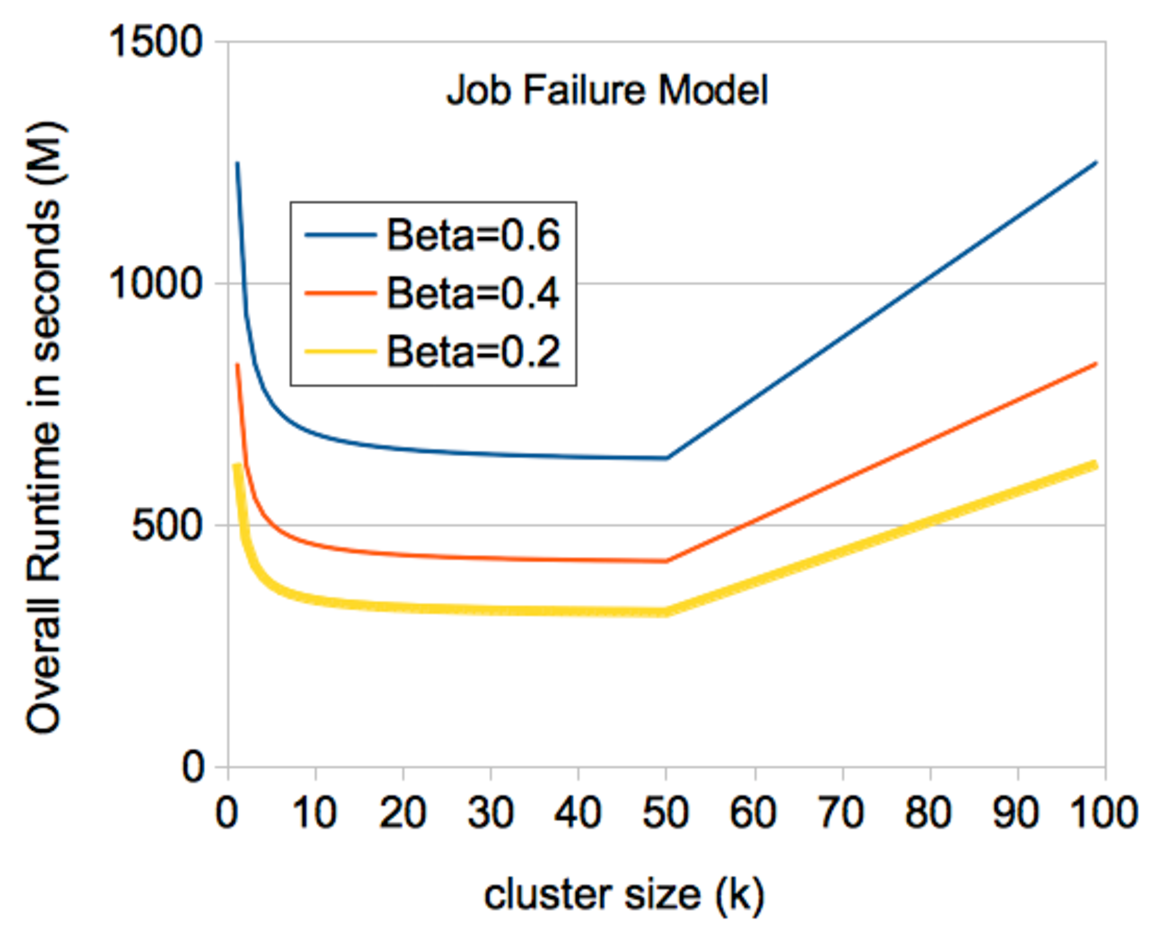
\includegraphics[width=0.6\textwidth]{figures/tolerance/ftc_jfm.pdf}
    \caption{Job Failure Model }
    \label{fig:ftc_jfm}
\end{figure}

 \begin{figure}[h!]
	\centering
    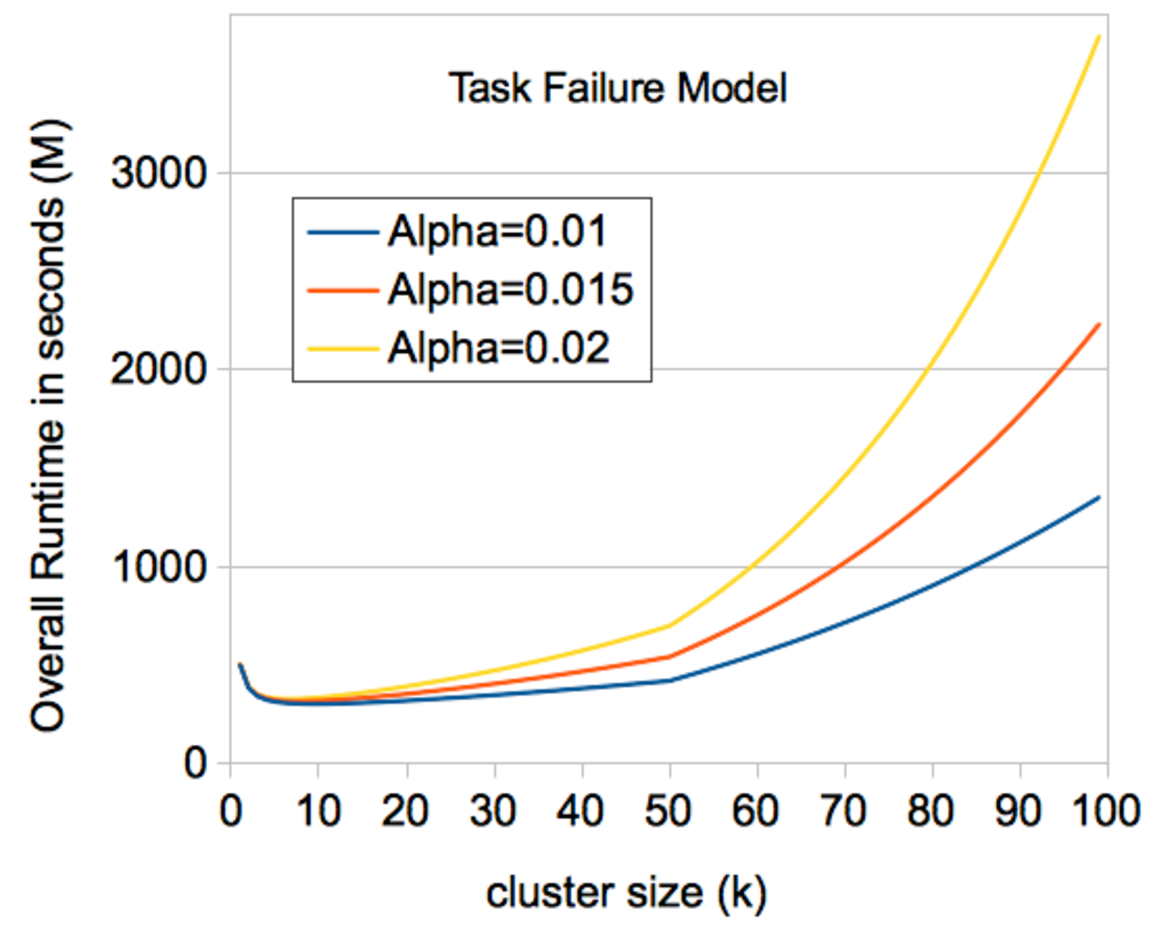
\includegraphics[width=0.6\textwidth]{figures/tolerance/ftc_tfm.pdf}
    \caption{Task Failure Model }
    \label{fig:ftc_tfm}
\end{figure}

\begin{figure}[h!]
	\centering
    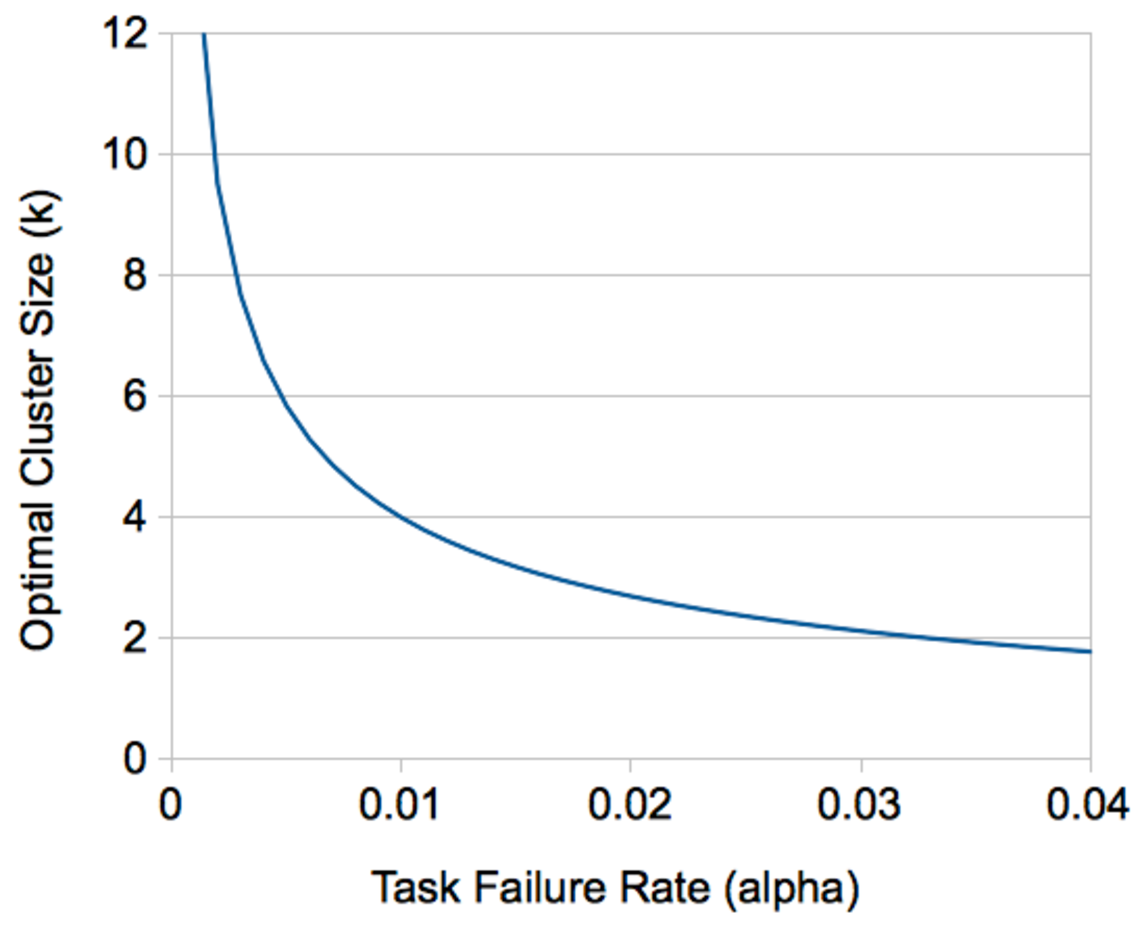
\includegraphics[width=0.6\textwidth]{figures/tolerance/ftc_relation.pdf}
    \caption{Task failure rate and optimal cluster size}
    \label{fig:ftc_relation}
\end{figure}
 
Figure~\ref{fig:ftc_relation} shows the relationship between the task failure rate and the optimal cluster size as indicated in Equation~\ref{eq:optimal1}. We can see that when the task failure rate is high ($\alpha>0.03$), it is better to abandon clustering ($\overset{*}{k}<1$).  We can also see that the optimal cluster size $\overset{*}{k}$ decreases with the increase of task failure rate. 

Below we introduce the method to tell which model a faulty environment belongs to if one has no knowledge about the cause of failures (transient or permanent, task or job). By analyzing the relationship between expected runtime and cluster size we can tell whether it tends to be TFM or JFM.  There are two criteria: 1) whether the overall runtime has an exponential increase (TFM) or a linear increase (JFM) when $k$ is large enough; 2) whether the optimal cluster size is influenced by the failure rates (If yes, TFM; otherwise JFM).
%We then apply TFM to the entire workflow. Although many implementation details have been ignored and especially the dependencies between jobs are disregarded, the experimental results show that such simplification is acceptable in practice. Also, we assume that the jobs in this workflow and the resources are homogeneous. The job-scheduling algorithm is First-Come-First-Serve, while one may use more complicated algorithms. 

From this theoretic analysis, we conclude that: 1) the lower the task failure rate is, the better runtime performance the task clustering has; 2) in TFM, adjusting cluster size according to the detected task failure rate can improve the runtime performance; 3) in JFM, we just need to set $k=n/r$. 

\subsection{Fault Tolerant Clustering Methods}
To improve the fault tolerance of horizontal clustering, we propose three methods: Dynamic Clustering (DC), Selective Reclustering (SR), and Dynamic Reclustering (DR). 

\begin{enumerate}
\item{Dynamic Clustering (DC)}

Dynamic Clustering adjusts the cluster size according to the task failure rate measured from jobs that have already been completed, either successfully or failed. 

\begin{figure}[h!]
	\centering
    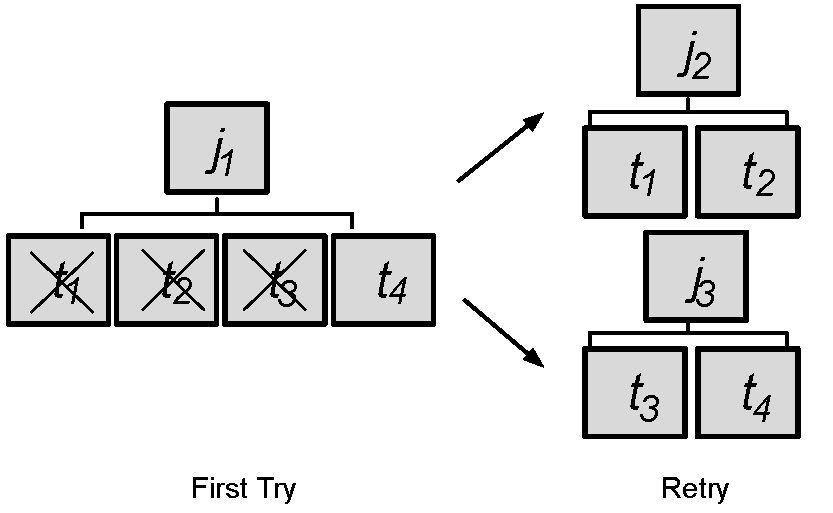
\includegraphics[width=0.6\textwidth]{figures/tolerance/ftc_dc.pdf}
    \caption{Dynamic Clustering}
    \label{fig:ftc_dc}
\end{figure}


%Failure records contain the information about the number of failed tasks, the type of tasks, the resource id, and a timestamp. The type of tasks is used to detect the task specific failures and the resource id is used to detect location specific failures. Then we calculate the average task failure rate and the average job failure rate. 
Figure~\ref{fig:ftc_dc} shows an example where the initial cluster size is 4 and thereby there are four tasks in a clustered job at the beginning. Then three out of these tasks fail. Assume that TFM suggests an optimal cluster size to be 2, then this job will be split into two clustered jobs while each has two tasks. The two clustered jobs are then submitted for retry.  DC is not aware that there are only three failed tasks. 

\item{Selective Reclustering (SR)}

In DC, one knows the average task failure rate but the information about which tasks have failed is not available. In practice, it may be hard to identify the failed tasks, but if it is supported, we can further improve the performance with Selective Reclustering that selects the failed tasks in a clustered job and merges them into a new clustered job. SR is different to the naïve job retry in that the latter method retries all tasks of a failed job even though some of the tasks have succeeded. 
Figure~\ref{fig:ftc_sr} shows an example of SR. At the beginning, there are four tasks and three of them have failed. One task succeeds and exits. Only the three failed tasks are merged again into a new clustered job and the job is retried. This approach does not intend to adjust the cluster size, although the cluster size will be smaller and smaller naturally after each retry since there are less and less tasks in a clustered job. In this case, the cluster size has reduced from 4 to 3.

\begin{figure}[h!]
	\centering
    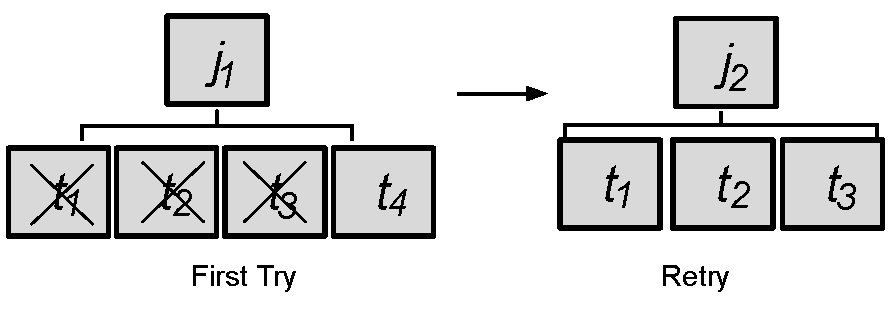
\includegraphics[width=0.6\textwidth]{figures/tolerance/ftc_sr.pdf}
    \caption{Selective Reclustering}
    \label{fig:ftc_sr}
\end{figure}


\item{Dynamic Reclustering (DR)}

Selective Reclustering does not analyze the failure rate and it uses a natural approach to reduce the cluster size if the failure rate is too high. However, it requires a special ability to select the failed tasks from all the tasks, while DC does not. We then propose the third method, Dynamic Reclustering, which is a combination of SR and DC to see whether using both strategies can improve the runtime performance of workflows further. In DR, only failed tasks are merged into new clustered jobs and the cluster size is also adjusted according to the detected task failure rate.
\begin{figure}[h!]
	\centering
    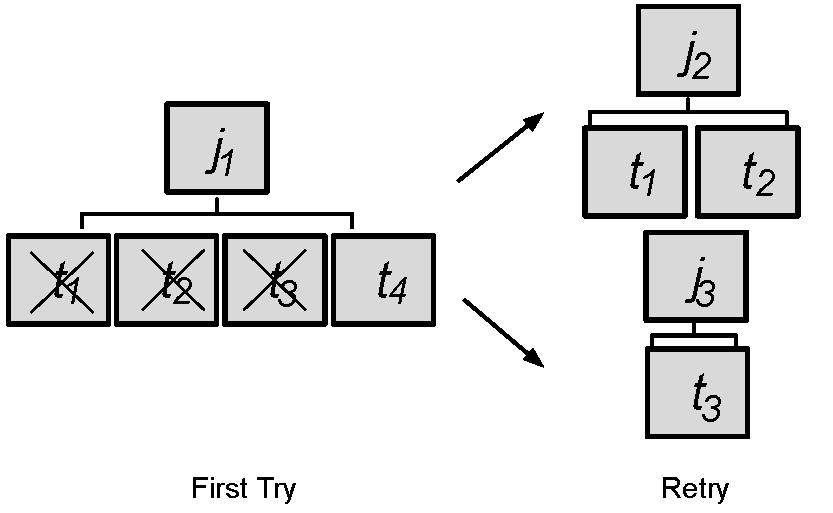
\includegraphics[width=0.6\textwidth]{figures/tolerance/ftc_dr.pdf}
    \caption{Dynamic Reclustering}
    \label{fig:ftc_dr}
\end{figure}


Figure~\ref{fig:ftc_dr} shows the steps of DR. At the last scheduling cycle, three tasks within a clustered job have failed. Therefore we have only three tasks to retry and further we need to adjust the cluster size (in this case it is 2) according to the task failure rate. 
\end{enumerate}



%We further improve our methods to be able to handle the situations where task failure rate is not fully independent of workflow characteristics or execution environment. Task specific failure is a type of failure that only occurs to some specific types of tasks. Location specific failure only occurs to some specific execution nodes. What is more, we present two refinements to handle the situation when there are fewer taskes than available resources. 

\section{Experiments and Discussion}

We use WorkflowSim \cite{WorkflowSim} to simulate these methods. Figure~\ref{fig:ftc_performance_1} compares the performance between DR and NOOP that has no optimization at all. Figure~\ref{fig:ftc_performance_1} shows that without any fault tolerant optimization, the performance degrades significantly especially when the task failure rate is high. Figure~\ref{fig:ftc_performance_2} compares the three methods that we proposed and it shows that Dynamic Reclustering outperforms the other two because it derives strengths from both. In reality, it is difficult to simulate failures with precise failure rates while WorkflowSim provides a unique platform to evaluate fault tolerant designs.

In conclusion of this section, for horizontal clustering, the first solution dynamically adjusts the cluster size according to the detected task failure rate. The second technique retries the failed tasks within a job. And the last solution is a combination of the first two approaches. 
\begin{figure}[!ht]
	\centering
    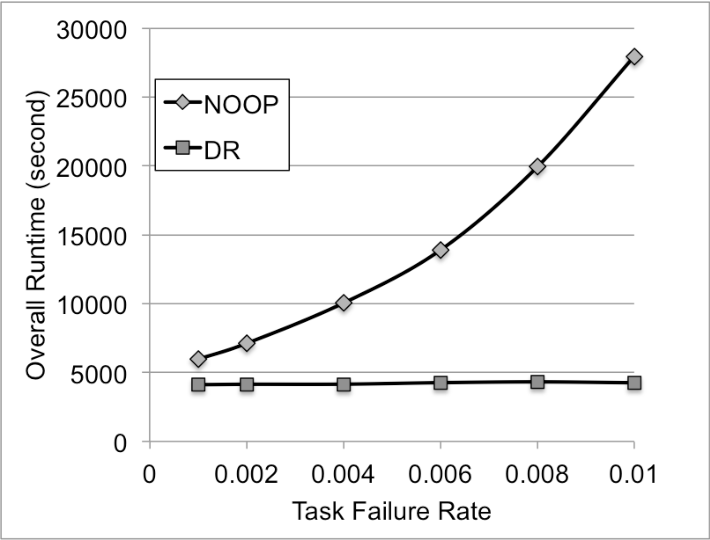
\includegraphics[width=0.5\textwidth]{figures/tolerance/ftc_performance_1.pdf}
    \caption{Performance between DR and NOOP}
    \label{fig:ftc_performance_1}
\end{figure}

\begin{figure}[!ht]
	\centering
    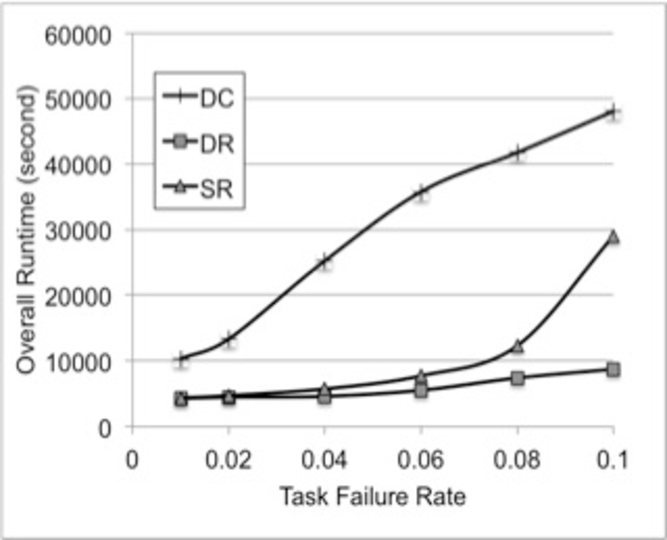
\includegraphics[width=0.5\textwidth]{figures/tolerance/ftc_performance_2.pdf}
    \caption{Performance between DC, SR, and DR}
    \label{fig:ftc_performance_2}
\end{figure}

%\section{Fault Tolerant Vertical Clustering}

%\begin{figure}[h!]
%	\centering
%   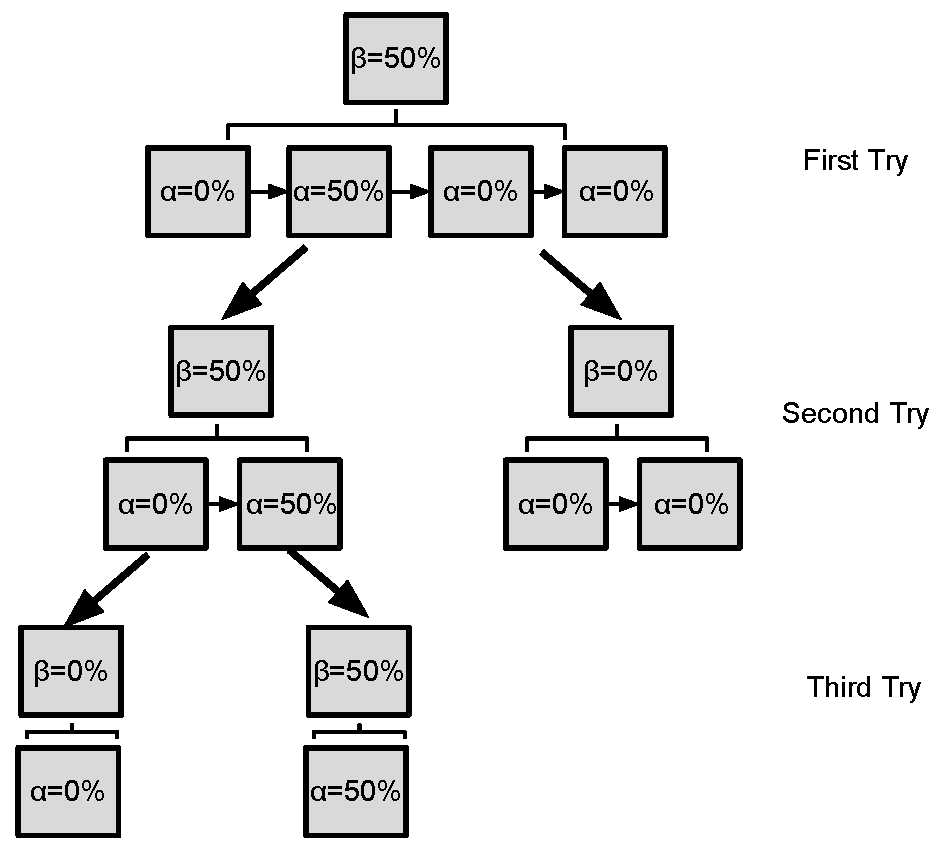
\includegraphics[width=0.7\textwidth]{figures/tolerance/ftc_bs.pdf}
%   \caption{Binary Search Method. The percentages are the task/job failure rates.}
 %  \label{fig:ftc_bs}
%\end{figure}
%For vertical clustering, we aim to merge as many tasks as possible if these tasks are not prone to fail and not to merge tasks at all if any task within the job may fail. Intuitively speaking, the failure of a parent task would cause a chain of failures of all of its child tasks and force all of them to retry, while in the case of non-clustering, we just need to retry the parent task and process its child tasks at the moment the parent task succeeds after retries. Such a dislike of failure-prone task in vertical clustering is more significant than that in horizontal clustering, in which the failure of a task does not influence another task since they have no data dependency. But typically, in a clustered job, tasks at different horizontal levels may have different task failure rates.

%To solve such a challenge, we propose a Binary Search (BS) method to identify the failure-prone tasks. The BS method merges all the tasks at the beginning since we do not have any prior knowledge of the failures. If the job failure rate is not zero, we decrease the cluster size by half and thus a failed job would be divided into two new jobs. If one type of the newly created job does not fail, it suggests that the failure-prone tasks are not in this part (at the same time it has been completed successfully). We just need to iterate these steps in the other part and eventually we divide the original clustered job into an appropriate set of small clustered jobs. 
%Figure~\ref{fig:ftc_bs} shows an example of four tasks while only the second one fails at a rate of 50\% and eventually it divides the workflow into three levels of clustered jobs. 

%In the future, we aim to evaluate this BS method on some widely used workflows and analyze its effectiveness. 

%Below we present heuristics to improve existing clustering strategies.

%In vertical clustering, tasks in the same pipeline can be merged into a new job. We use Epigenomics [20] as an example, which maps short DNA segments collected with high-throughput gene sequencing machines to a reference genome. Compared to Montage, Epigenomics has more parallel pipelines and thereby it is more suitable for vertical clustering. In Figure 12, a sample Epigenomics workflow has four pipelines and each has four tasks. We can set the cluster size to be 4 (maximum depth of each pipeline) and generate four merged jobs as shown below. In a fault environment, similarly to horizontal clustering, the overall runtime can be simplified as: (in this example, k is also the depth of a clustered job). 
                                                   
%If α>0,   increases exponentially with the increase of k; if α=0,   decreases with the increase of k. Such a feature suggests us to cluster as many tasks as possible if these tasks are not prone to fail but not to cluster at all if any task within the job may fail. Intuitively speaking, the failure of a parent task would cause a chain of failures of all of its child tasks and force all of them to retry, while in the case of non-clustering, we just need to retry the parent task and process the child tasks at the moment the parent task succeeds after retries. Such a dislike of failure prone task in vertical clustering is more significant than that in horizontal clustering, in which the failure of a task does not influence another task since they have no data dependency. But typically, in a clustered job, tasks at different horizontal levels may have different task failure rates. Eq. (6) suggests us to cluster failure-free tasks as much as possible but not to cluster any failure-prone tasks at all. 
